%%%%%%%%%%%%%%%%%%%%%%%%%%%%%%%%%%%%%%%%%%%%%%%%%%%%%%%%%%%%%%%%%%%%%%%%%%%%%%%%
% intro.tex: Introduction to the thesis
%%%%%%%%%%%%%%%%%%%%%%%%%%%%%%%%%%%%%%%%%%%%%%%%%%%%%%%%%%%%%%%%%%%%%%%%%%%%%%%%
% Outline:
% - Active matter and active fluids
% - Novel properties: rheology and diffusion
% - Collective phenomena: flocking and giant number fluctuations
%%%%%%%%%%%%%%%%%%%%%%%%%%%%%%%%%%%%%%%%%%%%%%%%%%%%%%%%%%%%%%%%%%%%%%%%%%%%%%%%




\chapter{Introduction}
\label{intro_chapter}
%%%%%%%%%%%%%%%%%%%%%%%%%%%%%%%%%%%%%%%%%%%%%%%%%%%%%%%%%%%%%%%%%%%%%%%%%%%%%%%%

\begin{itemize}

\item Chapter 1 briefly describe the history and significance of active fluid research.

\item Chapter 2 presents the experimental techniques used in this theis.

\item Chapter 3 talks about one of the emergent properties: reduced viscosity. Large portion of  this chapter have been published in \cite{Liu2019}.

\item Chapter 4 talks about another emergent property: giant number fluctuation. This work is under preparation for submission.

\item Chapter 5 presents the study on the transition from disordered state to active turbulence in light-powered bacterial suspensions. This work is conducted with a close collaboration with Yi Peng and Xiang Cheng. Large portions of this chapter has been published in \cite{Peng2020}. Yi Peng, Zhengyang Liu and Xiang Cheng conceived the experiment. Zhengyang Liu constructed the light-powered bacteria. Yi Peng performed the experiment. Zhengyang Liu and Yi Peng did the data analysis. All authors contribute to the model development and writing of the manuscript.

\item Chapter 6 summarizes the contributions of this thesis and provides the outlook on future research.

\item Appendix A shows details of the construction of light-powered \textit{E. coli}.

\item Appendix B provides details of several particle tracking tools I developed.

\item Appendix C shows details of photolithography.

\end{itemize}
%%%%%%%%%%%%%%%%%%%%%%%%%%%%%%%%%%%%%%%%%%%%%%%%%%%%%%%%%%%%%%%%%%%%%%%%%%%%%%%%


%%%%%%%%%%%%%%%%%%%%%%%%%%%%%%%%%%%%%%%%%%%%%%%%%%%%%%%%%%%%%%%%%%%%%%%%%%%%%%%%
\section{Active Matter and Active Fluids}
\label{active-fluids}

Active matter denotes a large group of active units which utilize ambient energy to achieve motions. Examples include flocking birds, schooling fish, herding beasts and even human crowds, down to actin filaments powered by motor proteins, bacteria and chemical reaction driven particles
\cite{Toner2005, Ramaswamy2010, Vicsek2012, Marchetti2013, Saintillan2013, Bechinger2016, Julicher2007}. The concept roots from a broader class of matter: soft matter, which includes polymers, surfactants and colloidal grains and shares common properties such as complexity and flexibility
\cite{DeGennes1992}. Like soft matter, active matter is also complex and flexible. What makes them more complex is the self-propulsion of each individual constituent, which endows them with more intrguing and counter-intuitive properties, challenging our understandings \cite{Glotzer2015}.

% such as abnormal rheology and emergent self-organized collective phenomena

Active fluids, sometimes referred to as active gels, are suspensions of active agents such as cells, particles and biological macromolecules that are capable of utilizing chemical energy to sustain their self-propulsion. They are a subset of active matter, and the "fluids" in the name suggests the important role of the viscous hydrodynamic interaction and stress, in contrast to dry active matter \cite{Marchetti2013}. The first glimmering of active fluids dates back to 1969, when Finlayson and Scriven found that motion could spontaneously set in a previously still material without the intervention of outside forces, due to composition-dependent stress \cite{Finlayson1969}. However, the study on active fluids did not bloom, until 26 year later, when the seminal paper on modeling collective flocks came out \cite{Vicsek1995}. From then on, physicists are getting unprecedentedly intereted in biological phenomena, leading to the emergence of a new field of study - active fluids.

Early accomplishments in the research of active fluids include two successful theoretical predictions on the abnormal rheology and the spontaneous active turbulence \cite{Hatwalne2004, Simha2002}, which were then demonstrated in quite a few experiments
\cite{Dombrowski2004, Wensink2012, Rafai2010, Sokolov2009, Gachelin2013, Lopez2015}. From these beginnings, the field has been enjoying a vibrant interplay between experiment and theory, and more complex environment and geometrical constraints have been investigated \cite{Ramaswamy2019}. As of now, the study of active fluids has provided us with a good qualitative understanding of some biological processes, such as how active turbulence enhances nutrient transport.

There are two promising directions in active fluids. One is to get quantitative understanding of the novel properties.  These works will not only provide more accurate predictions on new systems, but also guide the engineering of artificial robots that can perform tasks in complex environment, such as drug delivery. Another direction is to invite chemistry and biology to collaborate on this highly interdisciplinary subject. A complete understanding of the behavior and properties of living systems will require the knowledge of biochemical signaling, which opens the door of an ambitious mission: elucidating tissue dynamics and developmental biology \cite{Marchetti2013, Curatolo2020}. The works that are to be described in Sec.~\ref{rheology-of-bacterial-suspensions-under-confinement},
\ref{giant-number-fluctuations-in-3-dimensional-space} and \ref{the-emergence-of-active-turbulence} are along the first direction: seeking more quantitative understanding of rheology and active turbulence of active fluids.

\begin{figure}[!htbp]
	\begin{center}
	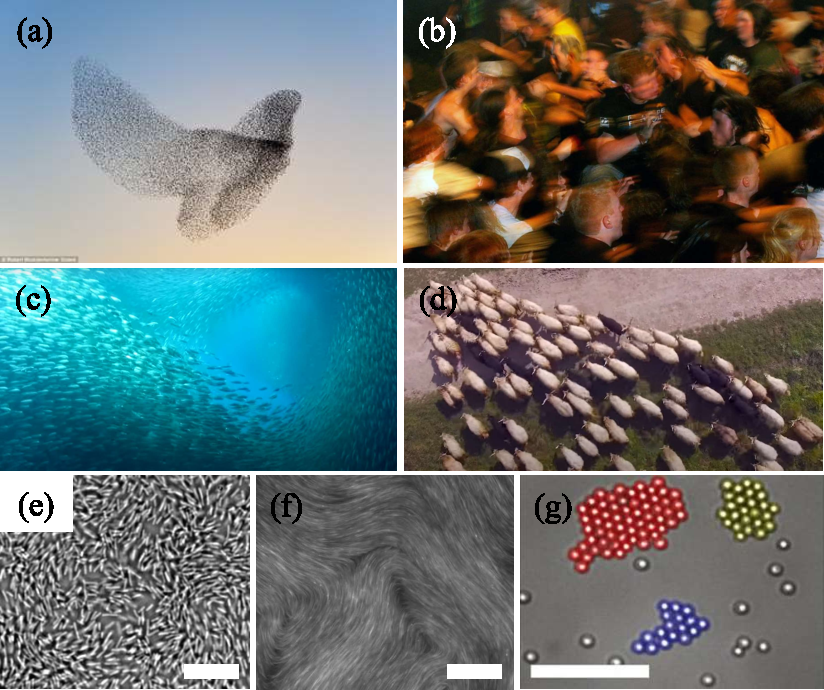
\includegraphics[width=5.5 in]{Figs/1-Intro/1.pdf}
	%select pdftexify command to run jpg or pdf files
	\end{center}
	\caption[Figure 1.1: ]
	{
	\textbf{Examples of living matters and active fluids.}
  (a) Flocking birds, (b) people in a mosh pit at heavy metal converts, (c) schooling fish, (d) herding sheeps, (e) swarming bacteria (f) microtubule and (g) clustering active Janus particles.
  Scalebars in (e) and (g) are 10 \textmu m. Scalebar in (f) is 200 \textmu m. Images courtesy of Robert Wolstenhome (a), Ulrike Biets (b) \cite{Silverberg2013}, biographic (c, d), DeCamp (f) \cite{DeCamp2015} and Palacci (g) \cite{Palacci2013}.
	}
	\label{fig:1-1}
\end{figure}

\section{Novel Properties}
\label{emergent-properties}
Active fluids exhibit novel properties such as reduced viscosity and enhanced diffusion  \cite{Ramaswamy2010}. The reduced viscosity is induced by the force excerted by the swimming mechanisms of the active agents, such as bacteria and algae \cite{Saintillan2018}. And the enhanced diffusion is attributed to the interaction - steric collision or hydrodynamic perturbation - between tracer particles and swimmers
\cite{Wu2000, Peng2016, Caspi2000, Morozov2014, Patteson2016, Leptos2009,
 Yang2016, Valeriani2011, Kurtuldu2011}.
In this section, the existing works regarding rheology and diffusion in active fluids are reviewed, and motivations for investigating the rheology of bacterial suspensions under confinement (Chap.~\ref{rheology-of-bacterial-suspensions-under-confinement}) will be discussed.


\subsection{Rheology}
\label{sec:rheology}
Viscosity of a fluid can be understood as its resistence to flow. When flowing, fluid elements move relative to others, resulting in energy dissipation due to friction. The more energy is required, the more "viscous" the fluid is known to be. A suspension
of passive particles is always more viscous than its suspending fluid, a fact that was first formulated by Einstein in 1906 \cite{Einstein1906}. Recently, the study of active fluids revealed that active particles modify the viscosity of their suspending fluids in a different and interesting way.

In 2004, Hatwalne et al. predicted that micro-swimmers, depending on their self-propelling mechanisms, can modify the suspension viscosity in different ways \cite{Hatwalne2004}. Most common micro-swimmers, such as unicellular microorganisms, can be classified into two types: pushers and pullers, based on the far field flow they generate. Fig.~\ref{fig:1-2}b illustrates the most common pushers and pullers in nature: bacterium and algae. If one puts a elongated rod-like bacterium in a simple shear flow, as illustrated in Fig.~\ref{fig:1-2}a, the preferred orientation of the bacterium is along the extensile flow \cite{Forster1974}. Such an orientation makes the flow generate by the swimming bacterium coincide with the imposed shear flow, and thus compensating the viscous dissipation of energy, which effectively reduces the viscosity. In contrast, in the case of puller swimmers, such an orientation makes opposites the directions of swimming induced flow and imposed shear flow, which enhances the visocity.

Their prediction was confirmed by numerical solutions of the theory \cite{Cates2008, Giomi2010} and experiments \cite{Sokolov2009, Gachelin2013, Lopez2015}. Cates et al. reached at the same conclusions as Hatwalne et al. did: while contractile gels exhibit a divergence of apparent viscosity, extensile gels show a zero-viscosity phase. Giomi et al., on top of these results, emphasized the important role of particle shape. They showed, in their numerical study, an rheological equivalence between rod-like pusher swimmers and disk-like puller swimmers (see Fig.~\ref{fig:1-2}c). In particular, they predicted a thickening effect of spherical puller swimmers (corresponds to the 0 shape parameter in Fig.~\ref{fig:1-2}c). This prediction was later on challenged by another theory in the framework of swim stress, which predicts a viscosity reduction of a spherical pusher swimmer suspension
\cite{Takatori2017}. Due to the difficulty of synthesizing large amount of artificial swimmers, this debate has not been resolved yet. However, with the rapid development of synthesizing techniques \cite{Palacci2013, Bricard2013}, it is getting more promising that we will resolve it, and formulate a more complete understanding on how active swimmers modify the rheology.

Experimental confirmation of these predictions posed challenges on traditional rheometries due to the tiny shear stress that is required to be measured. As a result, new rheometries are needed \cite{Marchetti2015}. In 2009, Sokolov and Aranson came up with an innovative way of measuring the such tiny stress \cite{Sokolov2009}. By moving a probe in a suspension of \textit{Bacillus subtilis} bacteria, a pusher type swimmer, they generated a large vortex. By studying the decay of the vortex, they got a measure of the viscosity. For the first time, they experimentally confirmed that pusher swimmers reduced the viscosity (see their results in Fig.~\ref{fig:1-2}d). In 2013, Gachelin et al. adopted a microfluidic viscometer to measure the viscosity of suspensions of \textit{Escherichia coli} bacteria, another pusher type swimmer \cite{Gachelin2013}. They confirmed again the viscosity reduction. A more remarkable finding is the non-newtonian behavior: the viscosity was reduced at low shear rate, but was enhanced at high shear rate. This observation suggested that it is the competation between bacterium intrinsic shear rate and the impose flow shear rate that determines how the viscosity is modified. In 2015, Lopez et al. published arguably the most important experimental work on the rheology of active fluids, which showed that the apparent viscosity of an \textit{E. coli} suspension can be reduced to zero if the swimming activity is sufficiently high \cite{Lopez2015}. The authors modified an old-fashioned Couette concentric cylinders, where the outer cylinder was set to rotate at a fixed rate and the torque on the inner cylinder was measured. The high sensitivity was achieved by using a string that was highly sensitive to torque to hang the inner cylinder, so that a stress, as small as that generated by bacterial suspensions, can be detected (see their rheometer and results in Fig.~\ref{fig:1-2}e-f). The authors termed their zero-viscosity suspensions ``superfluids''.

Despite the great progress on the rheology of active fluids made so far, their remained complexity that are not readily understood. Confinement, or more generally boundary conditions or geometry, is one of the leading factors that contribute to this complexity. The behavior of active particles can be altered greatly by confinement. In 2005, Voituriez et al. showed theoretically that a spontaneous flow transition from a homogeneous immobile state could happen in active polar gel under confinement \cite{Voituriez2005}. Such spontaneous flow transition was confirmed in both numerical and experimental studies \cite{Ravnik2013, Wioland2016, Wu2017}. The complexity introduced by geometry was also manifested by the experiments where single bacterial vortex was stabilized by confinement \cite{Woodhouse2012, Wioland2013, Lushi2014} and where asymmetric gears were powered by swimming bacteria
\cite{Sokolov2010, Hamby2018}. The effect of confinement on the rheology of active fluids was first studied theoretically based a kinetic theory \cite{Alonso-Matilla2016} and a generalized Navier-Stokes model \cite{Slomka2017}. In this thesis, I will present the first experimental study on active fluid rheology using bacterial suspensions
(Chap.~\ref{rheology-of-bacterial-suspensions-under-confinement}). The fact that our experimental results agreed with neither theory manifested the complexity and the lack of understanding of active fluids. Together with the experimental results, we provided a heuristic model that qualitatively captured the rheological properties and hope to stimulate further theoretical studies on this matter.

\begin{figure}[!htbp]
	\begin{center}
	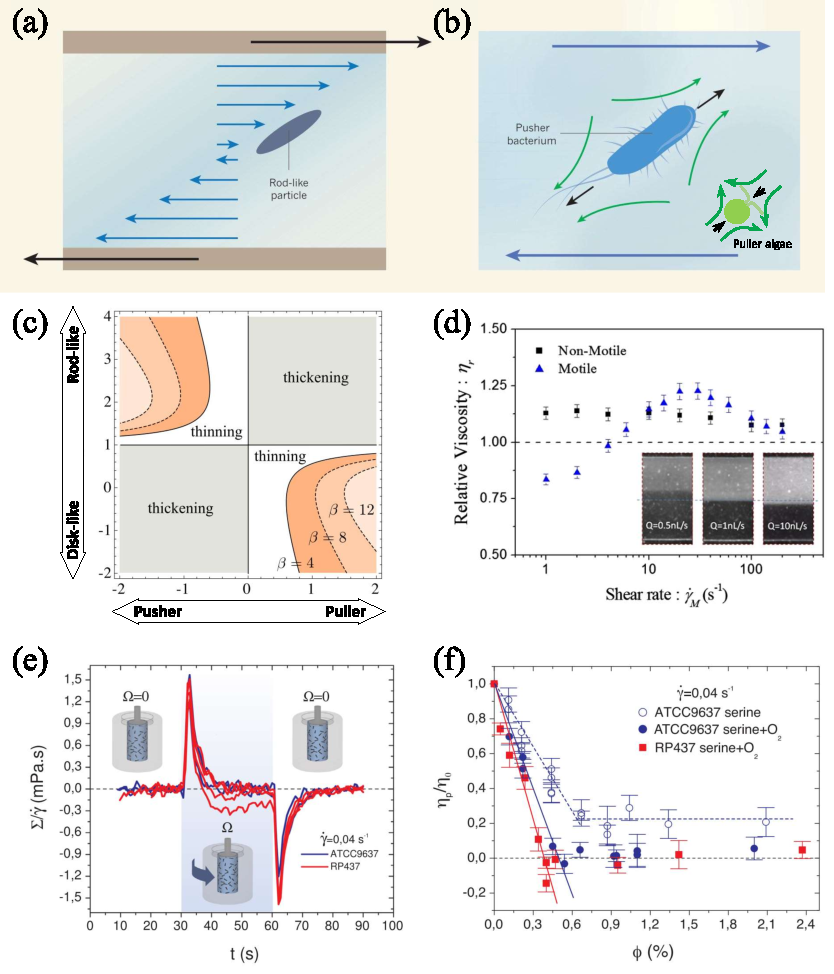
\includegraphics[width=5.5 in]{Figs/1-Intro/2.pdf}
	%select pdftexify command to run jpg or pdf files
	\end{center}
	\caption[Figure 1.2: ]
	{
	\textbf{Rheology of active fluids.}
	(a) The preferred orientation of the bacterium is along the extensile flow.
	(b) The most common pushers and pullers in nature: bacterium and algae, and their corresponding far field flow.
	(c) Rheological effect phase diagram of swimmer shape and swimming mechanism.
	(d) Non-Newtonian behavior of \textit{E. coli} suspensions.
	(e) Stress response of \textit{E. coli} suspensions in a modified Couette concentric cylinder rheometer.
	(f) Viscosity of \textit{E. coli} suspensions at various volume fractions.
	Image courtesy of Marchetti (a, b) \cite{Marchetti2015}, Giomi (c) \cite{Giomi2010}, Gachelin (d) \cite{Gachelin2013} and Lopez (e, f) \cite{Lopez2015}.
	}
	\label{fig:1-2}
\end{figure}


\subsection{Diffusion}
\label{sec:diffusion}
The diffusion of passive particles in active fluids, such as nutrients and signaling molecules, are significantly enhanced. Such enhancement has been shown to have great biological and ecological importance \cite{Wu2000, Kurtuldu2011, Morozov2014}, as well as to provide a useful tool of probing novel properties of active fluids \cite{Squires2010}. Unlike the study of rheology, which was initiated by theoretical prediction, the study of enhanced diffusion started from an experiment.

In 2000, Wu and Libchaber studied the diffusion of spherical polystyrene particles in a bath of actively swimming \textit{E. coli} \cite{Wu2000} (see Fig.~\ref{fig:1-3}a for their experimental system). They characterized the diffusion of the tracer particles by measuring their means squared displacement (MSD) (see Fig.~\ref{fig:1-3}b for typical MSD data), and reported two findings: 1) the MSD exhibits a superdiffusive regime at short time, which is followed by a diffusive regime at longer time; 2) the effective temperature, backed up from effective diffusion coefficient using Stokes-Einstein equation, is several order of magnitude larger than room temperature. Their qualitative findings were confirmed by computational \cite{Underhill2008, Lin2011}, theoretical \cite{Golestanian2009} and other experimental studies
\cite{Chen2007, Leptos2009, Mino2011, Kurtuldu2011, Patteson2016}. A remarkable progress towards quantitative understanding was made by Mino et al., who experimentally identified that the enhancement of diffusivity is proportional to the "activity flux" (defined as concentration multiplied by the mean velocity of swimmers). This model was further developed to capture the experimental result more accurately and to account for more complex conditions \cite{Mino2013, Kasyap2014, Morozov2014}.

Although a lot of progress has been made on understanding diffusion isotropic particles (spheres) in an active bath, how anisotropic particles diffuse remained largely unexplored. Yet, the diffusion of anisotropic particles has both fundamental and application significance. On the one hand, it was shown that the Brownian motion (i.e. in a passive bath) of anisotropic particles exhibited a subtle interplay between orientational and translational motions \cite{Han2006}. Previous studies preferred to consider an active bath equivalent to a high temperature passive bath \cite{Wu2000}, and it was shown to be a good equivalence for isotropic particles. A fundamentally interesting question to ask is: does active bath also alters the interplay between orientational and translational motions? The answer is yes, and we will see that this interplay is specific to swimming mechanisms. On the other hand, few particles or molecules in nature are perfectly isotropic. Generalizing the enhanced diffusion to anisotropic particles will have significant impact on applying this knowledge on real world problems. In 2016, Peng et al. studied the diffusion of polystyrene ellipsoids in a quasi-2D free-standing soap film of \textit{E. coli} bath (see setup schematic in Fig.~\ref{fig:1-3}c) \cite{Peng2016}. In contrast to the pure Brownian motion, where ellipsoids preferred to diffuse along their major axes \cite{Han2006}, they found that an active bath forced
the ellipsoids to move primarily along the minor axes (see Fig.~\ref{fig:1-3}d-e for a comparison). This phenomenon was explained by considering the far-field dipole flow of a single \textit{E. coli} bacterium. An interesting prediction naturally arises: in a bath of puller swimmers, whose far-field flow is opposite to that of pushers, the diffusion of ellisoidal tracers should be primarily along the major axes. This prediction was later on proved experimentally by Yang et al. \cite{Yang2016} in a green algae \textit{C. reinhardtii} bath and I was involved in this work. Due to the fact that my contribution was relatively small to this work, I will not provide more details about it in my thesis. However, readers interested are encouraged to find out more in our original paper \cite{Yang2016}.

\begin{figure}[!htbp]
	\begin{center}
	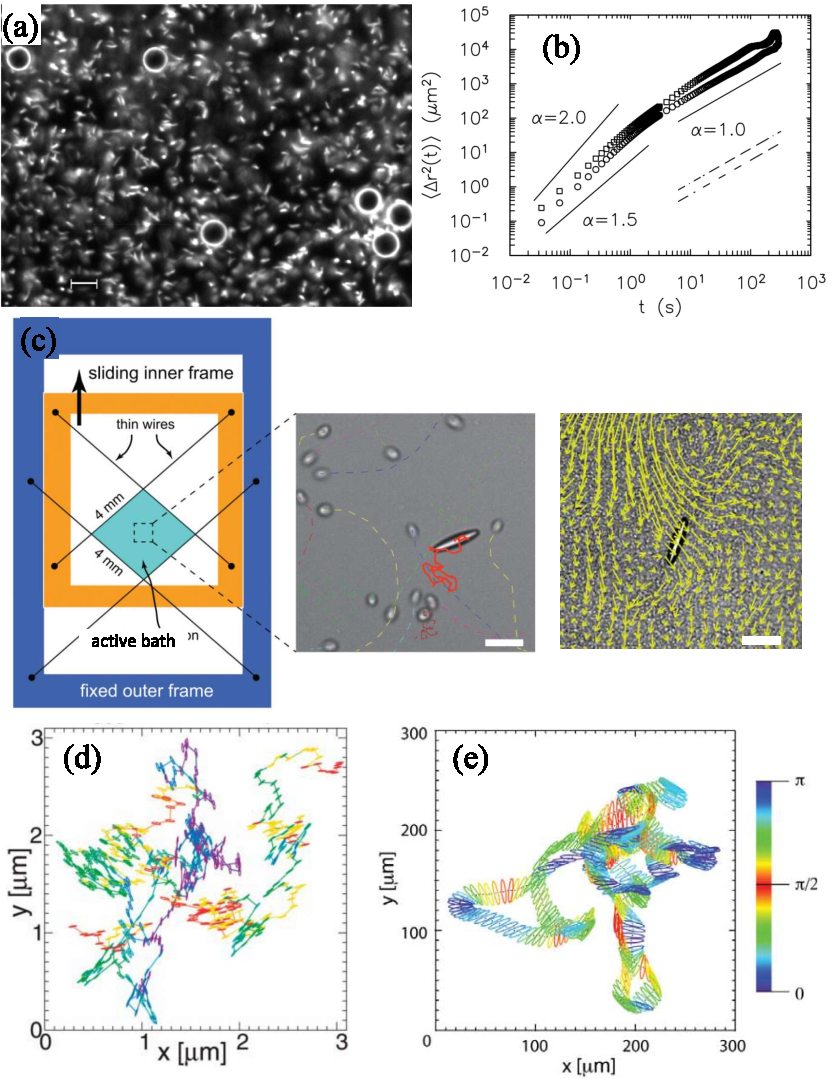
\includegraphics[width=5.5 in]{Figs/1-Intro/3.pdf}
	%select pdftexify command to run jpg or pdf files
	\end{center}
	\caption[Figure 1.3:]
	{
	\textbf{Diffusion of passive tracers in an active bath.}
	(a) 10 \textmu m diameter PS particles suspended in a bath of \text{E. coli}
	(b) Mean squared displacement (MSD) of tracer paticles as a function of lag time.
	(c) Free-standing film setup adopted by Peng et al. and Yang et al. (left)\cite{Peng2016, Yang2016}. A microscopic image of ellipsoidal PS particle suspending in \textit{C. reinhardtii} (middle) and \textit{E. coli} (right) baths. Scale bar: 20 \textmu m.
	(d) and (e) present both the translational and orientational trajectories of ellipsoids diffusion in water and \textit{E. coli} bath, respectively.
	Image courtesy Wu (a, b) \cite{Wu2000}, Yang (c) \cite{Yang2016}, Han (d) \cite{Han2006} and Peng (e) \cite{Peng2016}.
	}
	\label{fig:1-3}
\end{figure}



\section{Collective Motion and Giant Number Fluctuations}
Collective motion is defined as an emergent directed movement in a large number of animals or particles, which are capable of moving on their own.




\subsection{Collective Motion}
The research on collective phenomena dates back to the 1980s, when flocking birds, schooling fish, herding beasts and even human crowds (Fig.~\ref{fig:1-1}a-d) were regarded as an orientationally ordered phase of living matter, in analogy with ferromagnetic spins
\cite{Reynolds1987, Vicsek1995, Narayan2007, Ward2008, Ballerini2008, Silverberg2013}. This idea has since evoked enormous research interest on this seemingly universal animal behavior and its consequences. In this section, we first review recent progresses on understanding the collective phenomena in various living systems and motivate our research on "imaging the emergence of active turbulence"
(detailed in Chap.~\ref{the-emergence-of-active-turbulence}). Then, I will switch to an important consequence of the collective phenomena: giant number fluctuations, where I will motivate our research on "giant number fluctuations in 3-dimensional bacterial suspensions" (detailed in Chap.~\ref{giant-number-fluctuations-in-3-dimensional-space}).

Besides macroscopic systems mentioned above, smaller and more laboratory accessible model systems have joined this family and have been studied extensively. As examples, actin filaments and bacteria exhibit turbulence-like swirling patterns, and synthetic active colloids form dynamic clusters (Fig.~\ref{fig:1-1}e-g)
\cite{Dunkel2013, Wensink2012, Buttinoni2013, Palacci2013, Sanchez2012, Schaller2010, Sokolov2007}. As of today, these universal patterns can be qualitatively reproduced by simple models with collision rules and noise. And quantitative description is developing with more observations available, which is bound to have impactful applications, including understanding the reaction of panic crowd and predicting the migration of fish schools
\cite{Vicsek2012}.

Basic models Vicske model, continuum

Phase transitions

To test the prediction of the kinetic theory by Saintillan and Shelly, we perform experiment
\subsection{Giant Number Fluctuations}
Large scale inhomogeneity
